% SCRIPT
% The next project in this presentation is named "A Novel Strategy for Image Segmentation of Latent Fingerprints~}." 
% The results of this project were published on a confence paper in 2012. 
% Slide 1




% Slide 2


% Slide 3

% Conclusion

%\renewcommand{\Titulo}{A Novel Strategy for Image Segmentation of Latent Fingerprints~}


\begin{frame}{\citetitle{MarcoNuno_CongArbIng_2012_02_00} \footnotemark (1)}

\note[item]{\scriptsize  A Fingerprint is an impression or mark made on a surface by a person's fingertip, especially as used for identifying individuals from the unique pattern of whorls and lines.}
\note[item]{\scriptsize  The main stages of AFIS involves:  1. Capture of the fingerprint image. 2. Image processing 3. Feature extraction  4. Matching 5. Storing}
%\note[item]{\scriptsize  The adequate processing of the fingerprint image is a relevant task for the recognition process. If the image is not processed correctly, false characteristics could be obtained in the feature extraction phase or important information could be discarded, increasing the probability that the identification of the individual and the system fails.}
\note[item]{\scriptsize  In this project a new strategy for segmentation of latent fingerprints is proposed, based on the use of gradients and the detection of regions in the image. Our algorithm is able to detect the area of interest in the fingerprint eliminating spots, shadows, noise, etc., and adapting itself to the different conditions in the image.}

	\begin{itemize}
\item Automatic Fingerprint Identification Systems (AFIS) are very important due to their security applications.
\item The main stages of AFIS involves several image processing operators. 
\item The adequate processing of the fingerprint image is important 

	\end{itemize}
	    \begin{center}
    \begin{tabular}{c}
        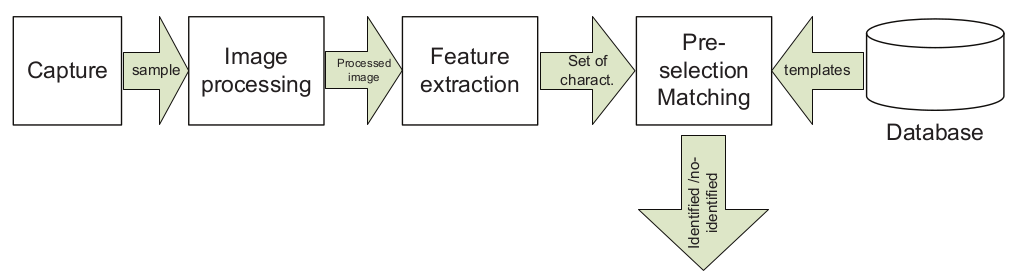
\includegraphics[width=0.75\linewidth]{Figs/Fingerprint1}\\
    \end{tabular}
    	    \end{center}

\footnotetext[1]{\fullcite{MarcoNuno_CongArbIng_2012_02_00}}
\setcounter{footnote}{0}
\end{frame}

\begin{frame}{\citetitle{MarcoNuno_CongArbIng_2012_02_00} (2)}
Estrategia propuesta:
\begin{columns}
		\begin{column}{0.48\textwidth}

		    \begin{enumerate} \small
		        \item Compute gradient and gradient magnitude.
                \item Normalize the pixel values to the range [0 255].
                \item Binarize the normalized image.
                \item Apply a mean filter to the binarized image            
            \end{enumerate}  
        \end{column}          
		\begin{column}{0.48\textwidth}
		    \begin{enumerate} \small
				\setcounter{enumi}{4}
    \item Binarize the image obtained
                \item Find the label matrix.
                \item Find the label with the high number of instances.
                \item Detect the largest region of interest.			
            \end{enumerate}  

        \end{column}
\end{columns}


\note[item]{\scriptsize  The gradient is a tool widely used for detecting edges in
an image. 
}

%\note[item]{\scriptsize This normalization is performed executing the following steps: ii) Find the minimum intensity value. ii) Subtract the minimum intensity value to each pixel in the image. iii) Find the maximum intensity value in the image and divide 255 by it. iv) Multiply each intensity value by the result obtained in the previous step.}

\note[item]{\scriptsize Binarize the normalized image using as threshold the
mean value of the gradient magnitude image.}

%\note[item]{\scriptsize A new median value is computed from the binarized image, which will be used as threshold for future binarization}

\note[item]{\scriptsize  The labeling algorithm allows to identify zones in the input image formed by interconnected pixels in a binary image that belongs to the foreground (object of interest).}

%\note[item]{\scriptsize Excluding labels that belongs to the background.}

%\note[item]{\scriptsize Send to the background the rest of the detected regions.}

		
\begin{center}
     \begin{tabular}{c}
         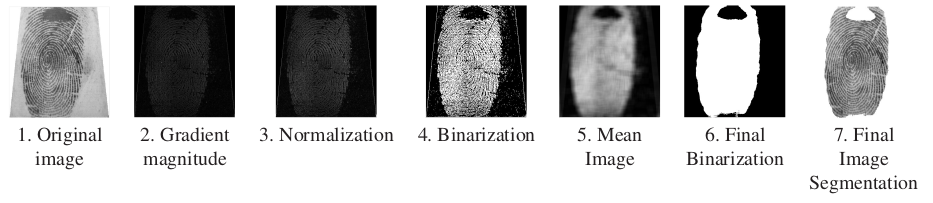
\includegraphics[width=0.95\linewidth]{Figs/Fingerprint2}\\
          \end{tabular}
\end{center}


\end{frame}

\begin{frame}{\citetitle{MarcoNuno_CongArbIng_2012_02_00} (2)}

\note[item]{\scriptsize  In this slide we show the different stages of the segmentation strategy proposed in this work. }

\note[item]{\scriptsize The resolution of images used in this work is 328 × 364 pixels .}

%Resultados
\begin{columns}
		\begin{column}{0.48\textwidth}
		We compared the proposed method against the most representative segmentation algorithms
		\begin{itemize}
		\item Our method achieves the better results, producing as result of
segmentation a single region and discarding no relevant information in the latent fingerprint.
    \item Images that have high contrast between the peaks and valleys that remark the borders in the image performs better.
				\end{itemize}
        \end{column}
				\begin{column}{0.48\textwidth}
				
\begin{center}
     \begin{tabular}{c}
              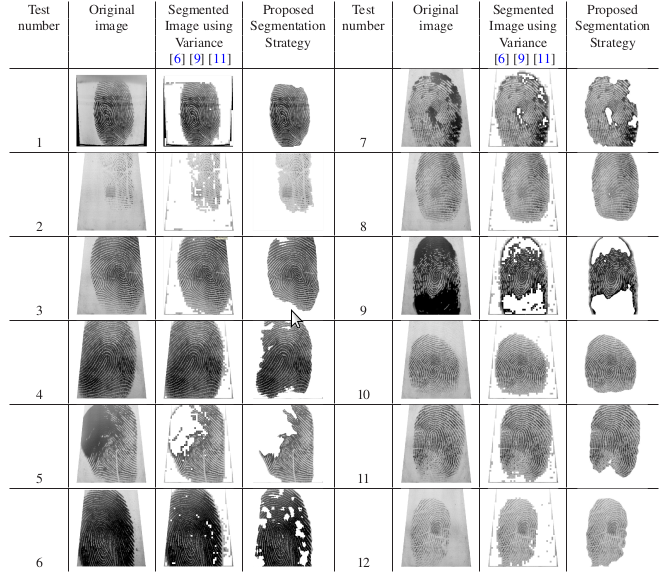
\includegraphics[width=0.85\textwidth]{Figs/Fingerprint3}
          \end{tabular}
\end{center}
				\end{column}
								\end{columns}

\end{frame}







